% Problem 2: LeNet-5 experiments and variants
\section{CNN Experiments (LeNet-style)}

\subsection{Design Decisions}
We implemented a baseline \texttt{LeNet5} with the following structure:
\begin{itemize}
  \item Input image: $28\times28\times1$
  \item Convolutional layer 1: $5\times5$, 6 filters $\rightarrow$ $24\times24\times6$
  \item Average pooling $2\times2$ $\rightarrow$ $12\times12\times6$
  \item Convolutional layer 2: $5\times5$, 16 filters $\rightarrow$ $8\times8\times16$
  \item Average pooling $2\times2$ $\rightarrow$ $4\times4\times16$
  \item Flatten $\rightarrow$ 256 features
  \item Fully connected layers: 256 $\rightarrow$ 120 $\rightarrow$ 84 $\rightarrow$ 10 logits
\end{itemize}

\begin{figure}[ht]
  \centering
  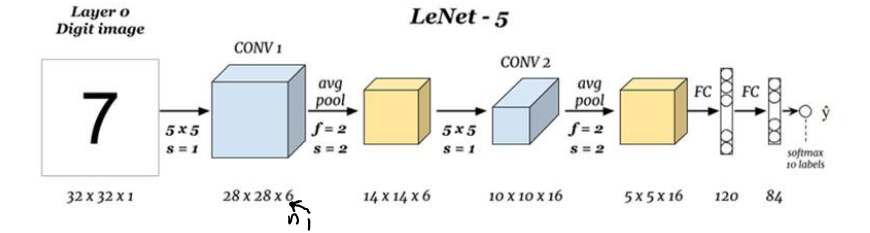
\includegraphics[width=0.6\linewidth]{../prob_2/Figures/lenet5.png}
  \caption{LeNet-5 architecture (baseline).}
  \label{fig:lenet}
\end{figure}

Variants added to investigate capacity and regularisation effects:
\begin{description}
  \item[Wide:]
  The spatial flow becomes:
  \begin{itemize}
    \item Input image: $28\times28\times1$
    \item Convolutional layer 1: $5\times5$, \textbf{16} filters $\rightarrow$ $24\times24\times\textbf{16}$
    \item Average pooling $2\times2$ $\rightarrow$ $12\times12\times\textbf{16}$
    \item Convolutional layer 2: $5\times5$, \textbf{32} filters $\rightarrow$ $8\times8\times\textbf{32}$
    \item Average pooling $2\times2$ $\rightarrow$ $4\times4\times\textbf{32}$
    \item Flatten $\rightarrow$ \textbf{512} features
    \item Fully connected layers: \textbf{512} $\rightarrow$ 120 $\rightarrow$ 84 $\rightarrow$ 10 logits
  \end{itemize}
  \item[Deep:]
  The spatial flow becomes:
  \begin{itemize}
    \item Input image: $28\times28\times1$
    \item Convolutional layer 1: $5\times5$, 6 filters $\rightarrow$ $24\times24\times6$
    \item Average pooling $2\times2$ $\rightarrow$ $12\times12\times6$
    \item Convolutional layer 2: $5\times5$, 16 filters $\rightarrow$ $8\times8\times16$
    \item Convolutional layer 3: $3\times3$, \textbf{32} filters $\rightarrow$ $8\times8\times\textbf{32}$
    \item Average pooling $2\times2$ $\rightarrow$ $4\times4\times\textbf{32}$
    \item Flatten $\rightarrow$ \textbf{512} features
    \item Fully connected layers: \textbf{512} $\rightarrow$ 120 $\rightarrow$ 84 $\rightarrow$ 10 logits
  \end{itemize}
  \item[Sigmoid:]
  Same as the baseline in terms of spatial sizes and feature dimensions, but with Sigmoid activations instead of ReLU.
\end{description}

Each variant is constructed by a factory function and run with the same training pipeline to ensure fair comparison.

\subsection{Parameters of the Experiment}
\begin{itemize}
  \item Learning rate: 0.001.
  \item Batch size: 128.
  \item Epochs: 5.
  \item Metrics: train accuracy, test accuracy, training wall time, testing wall time.
\end{itemize}

\subsection{Results and Findings}
The numerical outputs for the baseline and the three variants will be recorded in the consolidated tables below. Cells are left blank as placeholders to be filled with measured accuracies and times.

% ---- Consolidated Results Tables (placeholders) -------------------------
\begin{table}[ht]
  \centering
  \small
  \begin{tabularx}{\textwidth}{|l|*{6}{>{\centering\arraybackslash}X|}}
    \hline
    & \multicolumn{2}{c|}{DCT} & \multicolumn{2}{c|}{PCA} & \multicolumn{2}{c|}{AutoEncoder} \\
    \hline
    Classifier & Accuracy & Processing Time & Accuracy & Processing Time & Accuracy & Processing Time \\
    \hline
    K-means (k=1) & 0.9155 & 0.22174417 & 0.9165 & 0.11880670 &  &  \\
    K-means (k=4) & 0.9590 & 0.65419497 & 0.9595 & 0.62659590 &  &  \\
    K-means (k=16) & 0.9760 & 1.94901458 & 0.9775 & 1.66873733 &  &  \\
    K-means (k=32) & 0.9790 & 3.46641002 & 0.9775 & 2.53172698 &  &  \\
    SVM (Linear) & 0.9815 & 0.71919631 & 0.9785 & 0.59357043 &  &  \\
    SVM (Nonlinear) & 0.9855 & 1.84773630 & 0.9895 & 2.05351391 &  &  \\
    \hline
  \end{tabularx}
  \caption{Feature-based classifier results (placeholders).}
  \label{tab:features}
\end{table}

\vspace{6pt}

\begin{table}[ht]
  \centering
  \small
  \begin{tabularx}{\textwidth}{|l|*{6}{>{\centering\arraybackslash}X|}}
    \hline
    & \multicolumn{2}{c|}{DCT} & \multicolumn{2}{c|}{PCA} & \multicolumn{2}{c|}{AutoEncoder} \\
    \hline
    Variations & Accuracy & Processing Time & Accuracy & Processing Time & Accuracy & Processing Time \\
    \hline
    MLP (1-hidden) &  &  &  &  &  &  \\
    MLP (3-hidden) &  &  &  &  &  &  \\
    MLP (4-hidden) &  &  &  &  &  &  \\
    \hline
  \end{tabularx}
  \caption{MLP benchmark results (placeholders).}
  \label{tab:mlp}
\end{table}

\vspace{6pt}

\begin{table}[ht]
  \centering
  \small
  \begin{tabular}{|l|c|c|c|}
    \hline
    Variations & Accuracy & Training time & Testing time \\
    \hline
    Baseline &  &  &  \\
    Wide &  &  &  \\
    Deep &  &  &  \\
    Sigmoid &  &  &  \\
    \hline
  \end{tabular}
  \caption{CNN experiments summary (placeholders).}
  \label{tab:cnn}
\end{table}

% ---- End consolidated tables -------------------------------------------

\subsection{Discussion}
Discuss why the wide or deep variants behaved differently from baseline, how Sigmoid activation affected training dynamics, and any regularisation or optimisation observations (e.g., learning rate sensitivity).

\subsection{Conclusion and Recommendations}
Summarise best-performing variant, trade-offs between accuracy and compute (training time), and recommendations for further experiments (longer training, data augmentation, normalization).

% End of Problem 2
